\documentclass[letterpaper,11pt]{article}
\title{Boosting Algorithms and Overfitting : An empirical analysis}
\date{}
\author{Gaurav Kumar and Lakshmisha Bhat\\
  Johns Hopkins University\\
  \texttt{\{gkumar6,lbhat1\}@jhu.edu}}


\usepackage[margin=1in]{geometry}
% \usepackage{hyperref}
\usepackage[colorlinks]{hyperref}
\usepackage{capt-of}
\usepackage{amssymb}
\usepackage{amsmath}
\usepackage{url}
\usepackage{graphicx}
\usepackage{color}
\usepackage{bbm}
\usepackage{float}
\usepackage{graphicx}
\usepackage{wrapfig}
\usepackage{url}
\usepackage{wrapfig}
\usepackage{hyperref} 
\usepackage{color}
\usepackage{amstext}
\usepackage{enumerate}
\usepackage{amsmath,bm}
\usepackage{fullpage}
    
\renewcommand{\baselinestretch}{1.15}    

\everymath=\expandafter{\the\everymath\displaystyle}

\setlength{\abovecaptionskip}{1pt plus 0pt minus 0pt}
\setlength{\belowcaptionskip}{1pt plus 0pt minus 0pt}

\begin{document}
\large
\maketitle
\thispagestyle{headings}

\vspace{-.3in}

\thispagestyle{empty}

\begin{abstract}
We study the existing statistical views related to boosting, its behavior with respect to the bias-variance tradeoff and its rate of convergence with respect to the generalization error. We then perform an empirical study to confirm these views. These experiments use multiple datasets with different decision boundaries and we explore the change in accuracy of a boosted weak learner by varying training iterations and the size of the training dataset with varying noise levels. We also compare a boosted weak learner with various strong classifiers to find out if there is any merit in boosting a strong classifier. From these experiments we provide evidence for the fact that boosting is resistant to overfitting even with noisy training data sets. Finally, from these results we make a case for when boosting should be used and when not. 
\end{abstract}

\setcounter{secnumdepth}{-1} 

\section{Introduction}
Boosting \cite{s90} is a well-known, general method, for improving the accuracy of any given learning algorithm. It is known that Boosting is highly effective in obtaining a strong classifier from a set of weak predictors. Boosting algorithms construct high precision classifiers by taking a weighted combination of weak hypotheses, which do slightly better than random classification. It is also believed that Boosting algorithms like AdaBoost \cite{S99} are often robust to overfitting and reduce in-sample error to zero exponentially fast \cite{mrs}.

 Boosting is viewed as a method of applying sequential linear combinations of functions in a base hypothesis space \cite{BL98}. During each iteration the linear combination incorporates an additional term to optimize an objective function. Brieman \cite{BL98} made a path-breaking observation that the so called "unstable" methods can have their accuracy improved by "perturbing and combining" (P \& C), i.e, generate several versions of an estimator by perturbing the training set , and then combine several versions of the original into a single estimator. \cite{BL98} also introduces the definitions of bias and variance for a classifier as components of the out-of-sample error. It also provides a fundamental decomposition of the test set error of a classifier $C$ in terms of bayes classification error ($PE(C^*)$, minimum misclassification error achievable), bias and variance. 
\begin{align}
PE(C) = PE(C^*) + Bias (C) + Var (C) \nonumber
\end{align} 
where $PE(C)$ is the Generalization Error. This paper also made the first observation that boosting is a kind of gradient descent algorithm in function space (attributed to Brieman by Mason et al.'s 2000 paper).\\

Bagging \cite{BL98} and Boosting \cite{sfbl98} are different P\&C methods which were seen to be effectively reducing variance of the model by Brieman et al. Some of the evidence for this came from the observed effectiveness of "arcing" \cite{BL98} when used with C4.5 or CART, estimators known to have high variance. Since the error of these algorithms is mostly due to variance, the reduction in the error is hence due to a reduction in the variance. However, Schapire et al. \cite{sfbl98} disagree with this interpretation. They argue that while bagging is simply a variance reducing procedure, boosting can reduce both variance and bias collectively. They perform experiments (\cite{BL98} P 821) using decision stumps, which is a learning algorithm with very high bias. They conclude that using boosting on stumps actually " increases the variance, while at the same time it decreases the bias sufficiently to reduce the final error". These experiments clearly demonstrate that variance-reduction cannot explain the performance of boosting in its entirety. 

\section {Background}
\subsection {AdaBoost}
By far, the most popular example expressing the phenomenon that boosting is an additive/linear combination of  “weak” estimators is the AdaBoost algorithm \cite{S99}. 

\subsubsection {Training Error with AdaBoost}
"The most theoretical property of AdaBoost concerns its ability to reduce training error"  \cite{S99}. The training error of the final hypothesis is bounded by 
\begin{align}
\frac{1}{m}|\{ i:\text{  } H(x_i) \ne y_i\}| \le \frac{1}{m} \sum_i exp(-y_i f(x_i)) = \prod_t \mathcal Z_t \nonumber
\end{align}
where $f(x) = \sum_t \alpha_t h_t(x)$ so that H(x) = sign(f(x)). The above inequality follows from the fact that $e^{-y_i f(x_i)} \ge 1 \text{  if  } y_i \ne H(x_i)$. From the above equation one can deduce that the training error reduces rapidly if we chose an $\alpha_t$ and $h_t$ on each round to minimize $Z_t$, where \\
\begin{align}
\mathcal Z_t = \sum_i D_t(i) exp (-\alpha_t y_i h_t(x_i)) \nonumber
\end{align}
\begin{align}
D_t(i) = \text{ The weight of the distribution on a training example i} \nonumber
\end{align} 

\subsubsection {Generalization Error}
Freund and Schapire \cite{S99} initially showed that the bounds of the generalization error of the "aggregate learner" can be expressed in terms of the training error, the size $\it m$ of the sample, the VC-dimension $\it d$ of the "weak learner" and the number of training iterations $\it T$ of boosting. The generalization error was shown to be at most 
\begin{align}
\mathcal P[H(x) \ne y] + \bar O(\sqrt{\frac{Td}{m}}) \nonumber
\end{align}
\\
This generalization error bound suggests that boosting will overfit if run for too many rounds. This was later proved to be not necessarily true for all training datasets and sizes. This led Schapire et al. \cite{sfbl98} to give an alternative bound in terms of the margins of the training examples.

\subsection {Generalization error as a function of margin distributions}
The analysis based on "margin distributions" \cite{sfbl98} depend on the number of training examples and the ‘‘complexity’’ of the base classifiers, but do not depend explicitly on the number of base classifiers. The key idea of this analysis is that, in order to analyze the generalization error, one should consider the training error as well as the "confidence" of the predictions. The classification margin for an example is defined as the "difference between the weight assigned to the correct label and the $\it maximal $ weight assigned to any single incorrect label". The margin for an example (x,y) is defined to be
\begin{align}
\frac{y \sum_t \alpha_t h_t(x)}{\sum_t| \alpha_t|}
\end{align}
One can see that the margin is a number in the range [-1, 1] and that an example is classified correctly iff its margin is positive. A large positive margin is interpreted as a ‘‘confident’’ correct classification. However, the most critical result of their work is that boosting tends to increase the margins associated with examples and converges to a margin distribution in which "most" instances have large margins, especially by being aggressive in its effect on instances whose initial margin is small. So, the generalization error bound based on margins (which is entirely independent of training iterations T) is given by,
\begin{align}
\mathcal P [\text{  }margin_f(x,y) \text{  } \le \text{  } \theta] + \bar O(\sqrt{\frac{d}{m\theta^2}}) \nonumber \\
\text{ where } \theta > 0 \nonumber
\end{align}

Moreover, it is seen in most cases that AdaBoost  continues to reduce the generalization error even after the training error becomes zero. This is attributed to the fact that AdaBoost continues to increase the margins of the training examples without considering the attainment of zero training error as the evidence of convergence.

\section {Summary of current theoretical beliefs}
We list here some of the theoretical beliefs we attempt to verify using an empirical study. These are : 
\begin{enumerate}
\item Boosting reduces bias (and hence increases variance). \cite{bmw07}
\item Test accuracy while using a boosted weak learner is as good as learning with a strong classifier. \cite{s90}
\item AdaBoost will overfit if the number of training iterations is high enough. \cite{bmw07, BL98}
\item Boosting does overfit when the training data is noisy. \cite{klw01}
\end{enumerate}

\noindent
\section{Empirical Analysis of Boosting Algorithms}
The goal of this empirical analysis is to answer the following questions: 
\begin{enumerate}
\item	What are the implications of the choice of a weak base hypothesis on the test error?
\item	Given that Boosting reduces training error we see that there is in the past there has been no comparison made against the “true” error, the Bayes error. To what extent does AdaBoost reduce training error? Does it learn noise while doing so?
\item 	How does boosting perform with noisy training data?
\end{enumerate}

\subsection{Data Sets}
For the purpose of these experiments we chose to synthetically generate the datasets so as to control parameters like the noise, size of training and test datasets and the type of source distributions from which the data is sampled. We generate datasets with 100, 200, 400, 1000 and 2000 instances. We chose three datasets with the different decision boundaries as described below:
\begin{enumerate} 
\item Linearly Separable datasets : We choose a random linear separator by defining a random weight vector $w$. We chose to have ten possible features for all instances in the training and test datasets with two possible labels. We generate a random instance $x_i$ where $x_i \in X$, where $X$ is the set of instances. This random instance is created by generating random values for each of the features for the instance. We then use the following rule to generate class labels for the instance:
\begin{align}
y_i = \left\{ 
  \begin{array}{l l}
    A & \quad \text{if $w^Tx_i + b > 0$}\\
    B & \quad \text{otherwise}
  \end{array} \right.
\end{align}
where $b$ is a bias term. We now add $10\%$, $20\%$ and $30\%$ noise in the datasets by flipping the class label of the appropriate number of instances to generate the noisy datasets. 
\item Gaussian datasets : First we chose two distinct sets of gaussian distributions , where each gaussian distribution is valid for a certain feature. We have ten distinct gaussian distributions, one for each of the features for each possible label. Hence for each feature, and for each label there exists:
\begin{align}
\mathcal{N}_{kj}(\mu_{kj}, \sigma_{kj}) \text{   } \forall j \in F, k \in Y
\end{align}
where $F$ is the set of feature indices, and $Y = \{ A, B\}$ is the output space. We define, $\mathcal{N_A}$ as a mixture of the gaussian distributions $\mathcal{N_A}_i \text{   }\forall i \in F$ where each of these distributions are conditionally independent. 
We then generate random instances $x_i$ where $x_i \in X$ and $X$ is the set of instances in the following manner:
\begin{align}
y_i = \left\{ 
  \begin{array}{l l}
    A & \quad \text{if $x_i \in \mathcal{N_A}$}\\
    B & \quad \text{if $x_i \in \mathcal{N_B}$}
  \end{array} \right.
\end{align}

We now add $10\%$, $20\%$ and $30\%$ noise in the datasets by flipping the class label of the appropriate number of instances to generate the noisy datasets.
\item Spherical datasets : To generate this dataset we chose to use a 10-dimensional hyper-sphere where each dimension represents a feature. Hence this hyper-sphere exists in feature space. We generate random instances $x_i$ where $x_i \in X$ and $X$ is the set of instances, such that if the instance falls within the hyper-sphere then it has label $A$, otherwise it has label $B$. Let $r$ be the radius of the hyper-sphere. Then, 
\begin{align}
y_i = \left\{ 
  \begin{array}{l l}
    A & \quad \text{if $x_{ij} \le r \text{   } \forall j \in F$}\\
    B & \quad \text{otherwise}
  \end{array} \right.
\end{align}
We now add $10\%$, $20\%$ and $30\%$ noise in the datasets by flipping the class label of the appropriate number of instances to generate the noisy datasets.
\end{enumerate}

\pagebreak
\subsection{Experiments}
\subsubsection{Experiment1 : Classification Accuracy vs Training Iterations}  We start off by investigating how the performance of AdaBoost changes with the number of iterations it is allowed to run for. This experiment uses a C45 decision stump as the base classifier. We measure the change in accuracy for test (non-noisy) and train data sets with different levels of noise. We use 200 instances for the test dataset and 2000 instances to train. We then proceed to run this same experiment for all the data sets we had earlier generated, namely, the linear, spherical and the gaussian data sets. The results of these experiments are shown in Figure~\ref{fig:iterVsAccuracylinear} , Figure~\ref{fig:iterVsAccuracygaussian} and Figure~\ref{fig:iterVsAccuracyspherical}.
\begin{figure}[H]
  \centering
  \includegraphics[width=140mm]{iterVsAccuracy-linear.eps}
  \caption{Classification accuracy vs training iterations for Adaboost with a linear dataset.}
  \label{fig:iterVsAccuracylinear}
\end{figure}

\subsubsection{Conclusions from Experiment1}
\begin{enumerate}
\item With an increase in the number of iterations, AdaBoost does overfit the training data and hence the test error increases. This is apparent in the results from this experiment for all datasets. This behavior although significant, takes place very slowly with the increase in iterations. For examples, with a linear dataset with 10\% noise, the training error rate reduces from 10\% to 9\% in 10000 iterations. 
\item During the process of boosting for a large number of iterations, we do encounter an optimal solution even if the final solution is not the best possible one. This supports a similar claim made in \cite{Jiang01}.
\item The rate of increase of test error after the boosting algorithm achieves the best possible solution seems to be proportional to the noise in the training data set. 
\item The results from this experiment make a good case for early stopping which contradicts claims made in \cite{MW08}. 
\end{enumerate}

\begin{figure}[H]
  \centering
  \includegraphics[width=140mm]{iterVsAccuracy-gaussian.eps}
  \caption{Classification accuracy vs training iterations for Adaboost with a gaussian dataset.}
  \label{fig:iterVsAccuracygaussian}
\end{figure}

\begin{figure}[H]
  \centering
  \includegraphics[width=140mm]{iterVsAccuracy-spherical.eps}
  \caption{Classification accuracy vs training iterations of Adaboost with a spherical dataset.}
  \label{fig:iterVsAccuracyspherical}
\end{figure}

\subsubsection{Experiment2 : Classification Accuracy vs Size of Training set}  For this experiment we measure the change in performance of AdaBoost with variable training set sizes. This experiment uses a C45 decision stump as the base classifier and the number of iterations is fixed at 100. We measure the change in accuracy for test (non-noisy) and train data sets with different levels of noise. We then proceed to run this same experiment for all the data sets we had earlier generated, namely, the linear, spherical and the gaussian data sets. The results of these experiments are shown in Figure~\ref{fig:sizeVsAccuracylinear} , Figure~\ref{fig:sizeVsAccuracygaussian} and Figure~\ref{fig:sizeVsAccuracyspherical}.

\subsubsection{Conclusions from Experiment2}
\begin{enumerate}
\item With an increase in training set size, we see that the test error reduces consistently across all datasets. 
\item For the gaussian and the spherical datasets, the test error converges to close to zero values with about 1000 training samples, irrespective of the amount of noise in the training data.
\item Interestingly  enough, with the gaussian dataset, the test error starts increasing after hitting zero with 1000 training samples. 
\end{enumerate}

\begin{figure}[H]
  \centering
  \includegraphics[width=140mm]{sizeVsAccuracy-linear.eps}
  \caption{Classification accuracy vs size of Training set for Adaboost with a linear dataset.}
  \label{fig:sizeVsAccuracylinear}
\end{figure}

\begin{figure}[H]
  \centering
  \includegraphics[width=140mm]{sizeVsAccuracy-gaussian.eps}
  \caption{Classification accuracy vs size of Training set for Adaboost with a gaussian dataset.}
  \label{fig:sizeVsAccuracygaussian}
\end{figure}

\begin{figure}[H]
  \centering
  \includegraphics[width=140mm]{sizeVsAccuracy-spherical.eps}
  \caption{Classification accuracy vs size of Training set for Adaboost with a spherical dataset.}
  \label{fig:sizeVsAccuracyspherical}
\end{figure}

\subsubsection{Experiment3 : Classification Accuracy vs Iterations for various base classifiers}  In an attempt to justify the use of a weak learner instead of a strong one, we use various base classifiers with AdaBoost. The main idea is that if the test accuracy for the weak and the strong base classifiers with AdaBoost is comparable then we would rather use the weak classifier than the strong one. For this experiment we measure the change in performance of AdaBoost with change in training iterations. We use a C45 decision stump, a C45 Decision Tree with no depth limit, an SVM with a polynomial kernel (exponent 2) and a multi-layer perceptron with the number of hidden layers equal to half the number of features, as the base classifiers. We measure the change in accuracy for a non-noisy test data set and train data sets with 30$\%$ noise. We then proceed to run this same experiment for all the data sets we had earlier generated, namely, the linear, spherical and the gaussian data sets. The results of these experiments are shown in Figure~\ref{fig:modelVsAccuracytrainlinear} , Figure~\ref{fig:modelVsAccuracytraingaussian}, Figure~\ref{fig:modelVsAccuracytrainspherical}, Figure~\ref{fig:modelVsAccuracytestlinear} , Figure~\ref{fig:modelVsAccuracytestgaussian} and Figure~\ref{fig:modelVsAccuracytestspherical}.

\begin{figure}[H]
  \centering
  \includegraphics[width=140mm]{modelVsAccuracy-train-linear.eps}
  \caption{Training error for base classifiers vs iterations for Adaboost with a linear dataset}
  \label{fig:modelVsAccuracytrainlinear}
\end{figure}

Conclusions from Experiment3:
\begin{enumerate}
\item Boosting a C45 stump appears to always perform better in terms of test accuracy in comparison to boosting a C45 decision tree. 
\item When boosted, C45 decision trees and Multi-layer perceptrons are prone to over-fitting on linear and spherical datasets. 
\item The training error while using a boosted C45 stump seems to be always close to the true error of the training dataset. 
\item It is interesting to observe that on the linear dataset, an SVM does significantly better than a boosted C45 decision stump. This implies that the structure of the dataset affects how well boosting can work when compared with a stock strong classifier. 
\end{enumerate}

\begin{figure}[H]
  \centering
  \includegraphics[width=140mm]{modelVsAccuracy-train-gaussian.eps}
  \caption{Training error for base classifiers vs iterations for Adaboost with a gaussian dataset}
  \label{fig:modelVsAccuracytraingaussian}
\end{figure}

\begin{figure}[H]
  \centering
  \includegraphics[width=140mm]{modelVsAccuracy-train-spherical.eps}
  \caption{Training error for base classifiers vs iterations for Adaboost with a spherical dataset}
  \label{fig:modelVsAccuracytrainspherical}
\end{figure}

\begin{figure}[H]
  \centering
  \includegraphics[width=140mm]{modelVsAccuracy-test-linear.eps}
  \caption{Test error for base classifiers vs iterations for Adaboost with a linear dataset}
  \label{fig:modelVsAccuracytestlinear}
\end{figure}

\begin{figure}[H]
  \centering
  \includegraphics[width=140mm]{modelVsAccuracy-test-gaussian.eps}
  \caption{Test error for base classifiers vs iterations for Adaboost with a gaussian dataset}
  \label{fig:modelVsAccuracytestgaussian}
\end{figure}

\begin{figure}[H]
  \centering
  \includegraphics[width=140mm]{modelVsAccuracy-test-spherical.eps}
  \caption{Test error for base classifiers vs iterations for Adaboost with a spherical dataset}
  \label{fig:modelVsAccuracytestspherical}
\end{figure}

\section{Conclusion}
We show from our experiments that boosting a strong classifier has no significant benefits over boosting a weak learner. In most cases, it is preferable to use a weak classifier for boosting because of its speed and simplicity. In some cases however, using a stock strong classifier will yield better results than using a boosted C45 stump as we saw with Experiment 3. Hence, even though boosting is not a one-fit-all solution, since its rate of overfitting is slow and rate of convergence is fast (with early stopping), boosting is a good solution to explore before moving on to a stronger and more complex learner. 

%\listoffigures

\begin{thebibliography}{9}

\bibitem{s90}
   R. E. Schapire,
  \emph{The  Strength  of Weak Learnability}.
  Machine Learning,
  5, 197-227,
  1990.
\bibitem{sfbl98}
   R. E. Schapire and Y. Freund and P. Bartlett and W. S. Lee,
  \emph{Boosting the margin: A new explanation for the effectiveness of voting methods}.
  The Annals of Statistics,
  26, 1651-1686,
  1998.
\bibitem{mrs}
   I. Mukherjee and C. Rudin and R. E Schapire,
  \emph{The rate of convergence of adaboost}.
  JMLR W\&CP
\bibitem{hwwmj08}
   Gholamreza Haffari and Yang Wang and Shaojun Wang and Greg Mori and Feng Jiao
  \emph{Boosting with Incomplete Information}.
  ICML, 
  2008
\bibitem{cll12}
  Shang-Tse Chen and Hsuan-Tien Lin and Chi-Jen Lu
  \emph{An Online Boosting Algorithm with Theoretical Justifications}.
  ICML, 
  2012
\bibitem{byb09}
  B. Babenko and M. Yang and S. Belongie
  \emph{A Family of Online Boosting Algorithms}.
  3rd IEEE ICCV Workshop on On-line Learning for Computer Vision, 
  1346-1353, 2009a.

\bibitem{S99}
  Shapire, R. E.,
 \emph{ Theoretical views of boosting}.
  Computational learning theory,
  Fourth European Conference, EuroCOLT'99,1-10.

\bibitem{Jiang01}
  Wenxin Jiang ,
  \emph{ Some Theoretical aspects of Boosting in the presence of Noisy Data}
   , ICML 2001.

\bibitem{MW08}
  Mease , D., Wyner A.,
  \emph{ Evidence Contrary to the Statistical View of Boosting}
   , Journal of Machine Learning Research 9 (2008) 131-156.

\bibitem{BL98}
Brieman, L. (1998). 
\emph{Arcing classifiers}.
Ann. Statist. 26 801–849. MR1635406

\bibitem{fht00}
Jerome Friedman, Trevor Hastie, and Robert Tibshirani
\emph{Additive logistic regression: a statistical view of boosting }
, Ann. Statist. Volume 28, Number 2 (2000), 337-407.

\bibitem{bmw07}
Andreas Buja, David Mease, and Abraham J. Wyner
\emph{Comment: Boosting Algorithms: Regularization, Prediction and Model Fitting}
,Statist. Sci. Volume 22, Number 4 (2007), 506-512

\bibitem{klw01}
A Krieger, C Long, A J Wyner
\emph{Boosting noisy data}
,Proceedings of the Eighteenth International Conference on Machine Learning (2001)


\end{thebibliography}
\end{document}
